\section{Implementation \& Training}
\label{sec-implementation-and-training}

\subsection{Data Collection}
\label{sec-experiment-setting}
\begin{figure}
    \centering
    \subfigure[input from same environment]{
        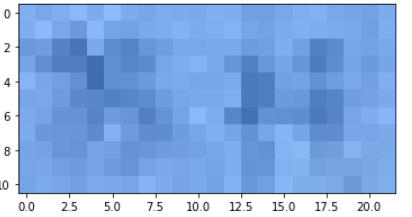
\includegraphics[width=0.2\textwidth]{pic/training_single_dataset_1.png}
        \label{fig-train-single-1}
        }
    \subfigure[output of (a)]{
        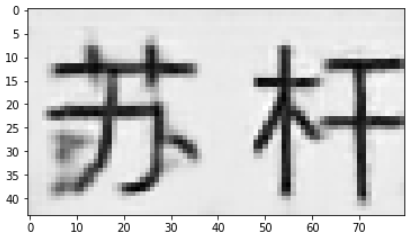
\includegraphics[width=0.2\textwidth]{pic/training_single_dataset_2.png}
        \label{fig-train-single-2}
        }
    \subfigure[input from different environment]{
        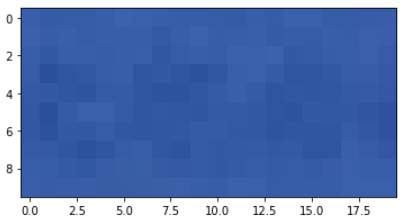
\includegraphics[width=0.2\textwidth]{pic/training_single_dataset_5.png}
        \label{fig-train-single-3}
        }
    \subfigure[output of (c)]{
        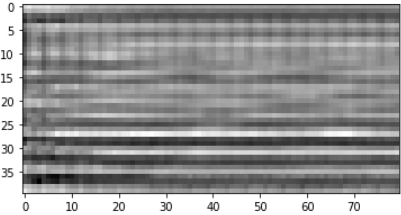
\includegraphics[width=0.2\textwidth]{pic/training_single_dataset_4.png}
        \label{fig-train-single-4}
        }
   % \subfigure[ground truth]{
    %    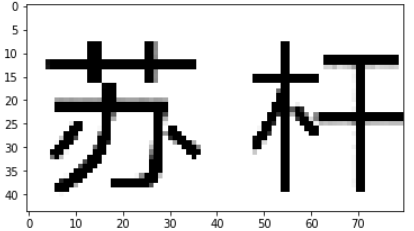
\includegraphics[width=0.2\textwidth]{pic/training_single_dataset_3.png}
     %   \label{fig-train-single-5}
      %  }
       \caption{Results of training with data collected in fixed environment. The network performs well in this environment but fails in other.}
       \label{fig-train-single}
\end{figure}

In our experiment, we are forced to collect the training dataset on our own instead of using public datasets. Because of our unique application, to the best of our knowledge there is no publicly available image dataset built for shoulder-surfing. Modern network architectures work with naturally obtained images, e.g. ordinary photos, satellite images, scanned documents, YouTube videos, etc. where the images are well focused and captured within the imaging ability of the camera, with the objects of interest, e.g. the face or the printed word, at least visible to the naked eye. and we apply the SR algorithms to reduce noise and refine details, like repainting texture and refining edges. However, as emphasized above, in our application we face images that is extremely blurred and distorted, due to the extreme circumstances when the photos are taken, and it is impossible to tell from each single picture whether a stroke of a character really belongs here, as it's equally possible that this line is a distorted mixture of multiple lines or is a mutilated part of a longer stroke. These are the reasons why our work does not choose datasets that are publicly available, and collect data by ourselves--as it will completely defeat the purpose if we turn to these datasets. And this also explains why we failed in trying to get comparable results with other SR architectures we use as baselines, as these networks are designed for another purpose and they hardly ever faced such distorted and blurred images.

The task of data collection is quite tedious, as we discovered that we need photos taken in all kinds of environments to train a robust network. We initially collect 60,000 images with the position of the smartphones static and all other environmental parameters stationary, and divided it into training and testing datasets which do not have common characters between them. Note that different lenses have different photographing abilities and blurring patterns, so the model has to be trained for each phone model. When using smartphones with optical zoom, the images will shift slightly time after time even if we keep them completely still, so the aligning phases are still needed (this shifting is also beneficial in that it simulates normal hand tremors in real-life scenarios even if we fix the phone to a stand instead of holding it up throughout the data collection phase which can last several hours). There is no consistency between adjacent images, so we also shuffle the images to increase this shifting effect and increase the variety of the training data. %To reduce calculation and better align the images with the ground truth, in the training data collection phase we drew a box around the text on the victim's screen, replacing the edges of the phone for alignment and cropping in the alignment step (as shown in Figure~\ref{fig-training}), but our system works perfectly without it.

Our network easily learned the patterns and presented equally satisfactory results in the test dataset (see Figure~\ref{fig-train-single-2}), displaying clean, easy to read results, showing that the network has learned to extract features beneath the character level, and it is highly possible that this network can recover all kinds of characters, not limited to the characters in the training dataset. However, when we slightly modified the environment, the images displaying the text with a different shade and size, none of the features were successfully extracted, and the network outputted white noise (see Figure~\ref{fig-train-single-4}).

\subsection{Experiment Setting}
As a result of these observations, we have to collect images in varied environments. Our experiment consists of 2 smartphones, one for the attacker and one the victim. Their distance is between 1 and 2 meters for traditional lenses (for the camera of the attacker's phone) without optical zooming, and 5 to 7.5 meters for lenses with optical zooming. Both phones are fixed to stands to keep them completely still, but as mentioned above, the lenses with optical zoom will shift slightly time to time, which is similar to a handheld situation. An app runs inside the attacker's phone, taking photos continuously, adjusting its focus and aperture, trying it's best to capture high-quality photos. Another app runs inside the victim's phone, displaying random characters with several fonts and colors, for the attacker to capture. The characters are selected from commonly used Chinese characters with 5 to 10 strokes and the English alphabet, and we divide this assemble into training and testing subsets. As the English characters are apparently easier to classify and reconstruct for the networks, the experiments testing the performance of the network will be performed only on Chinese characters, but it is our observation that our system works on English characters as well as Chinese characters.

As the experiment goes on, the attacker phone will keep on taking photos in burst mode (20 photos per time), and the victim phone will change the characters it is displaying at a fixed interval, when approximately 100 images were taken by the attacker. We change the environmental setting whenever about 2k photos were taken, relocating the phones (while keeping their distance between 1 and 2 meters) or modifying the angle of the phones. The attacker will always point its phone directly at the victim, keeping its screen in the middle of the photos; The victim, however, may tilt its phone at an angle within 30 degrees. We then readjust the focus and aperture of the attacker's phone to maximize the image quality before continuing data collection. Screenshots were taken in the victim's phone each time it changes its display, and these screenshots are scaled, spun and deformed according to the distance and angle between the phones at the time, and used as ground truth for training and evaluation. An illustration of our experimental setting is displayed in Fig.~\ref{illustration_of_system}.
\begin{figure}
	\centering
	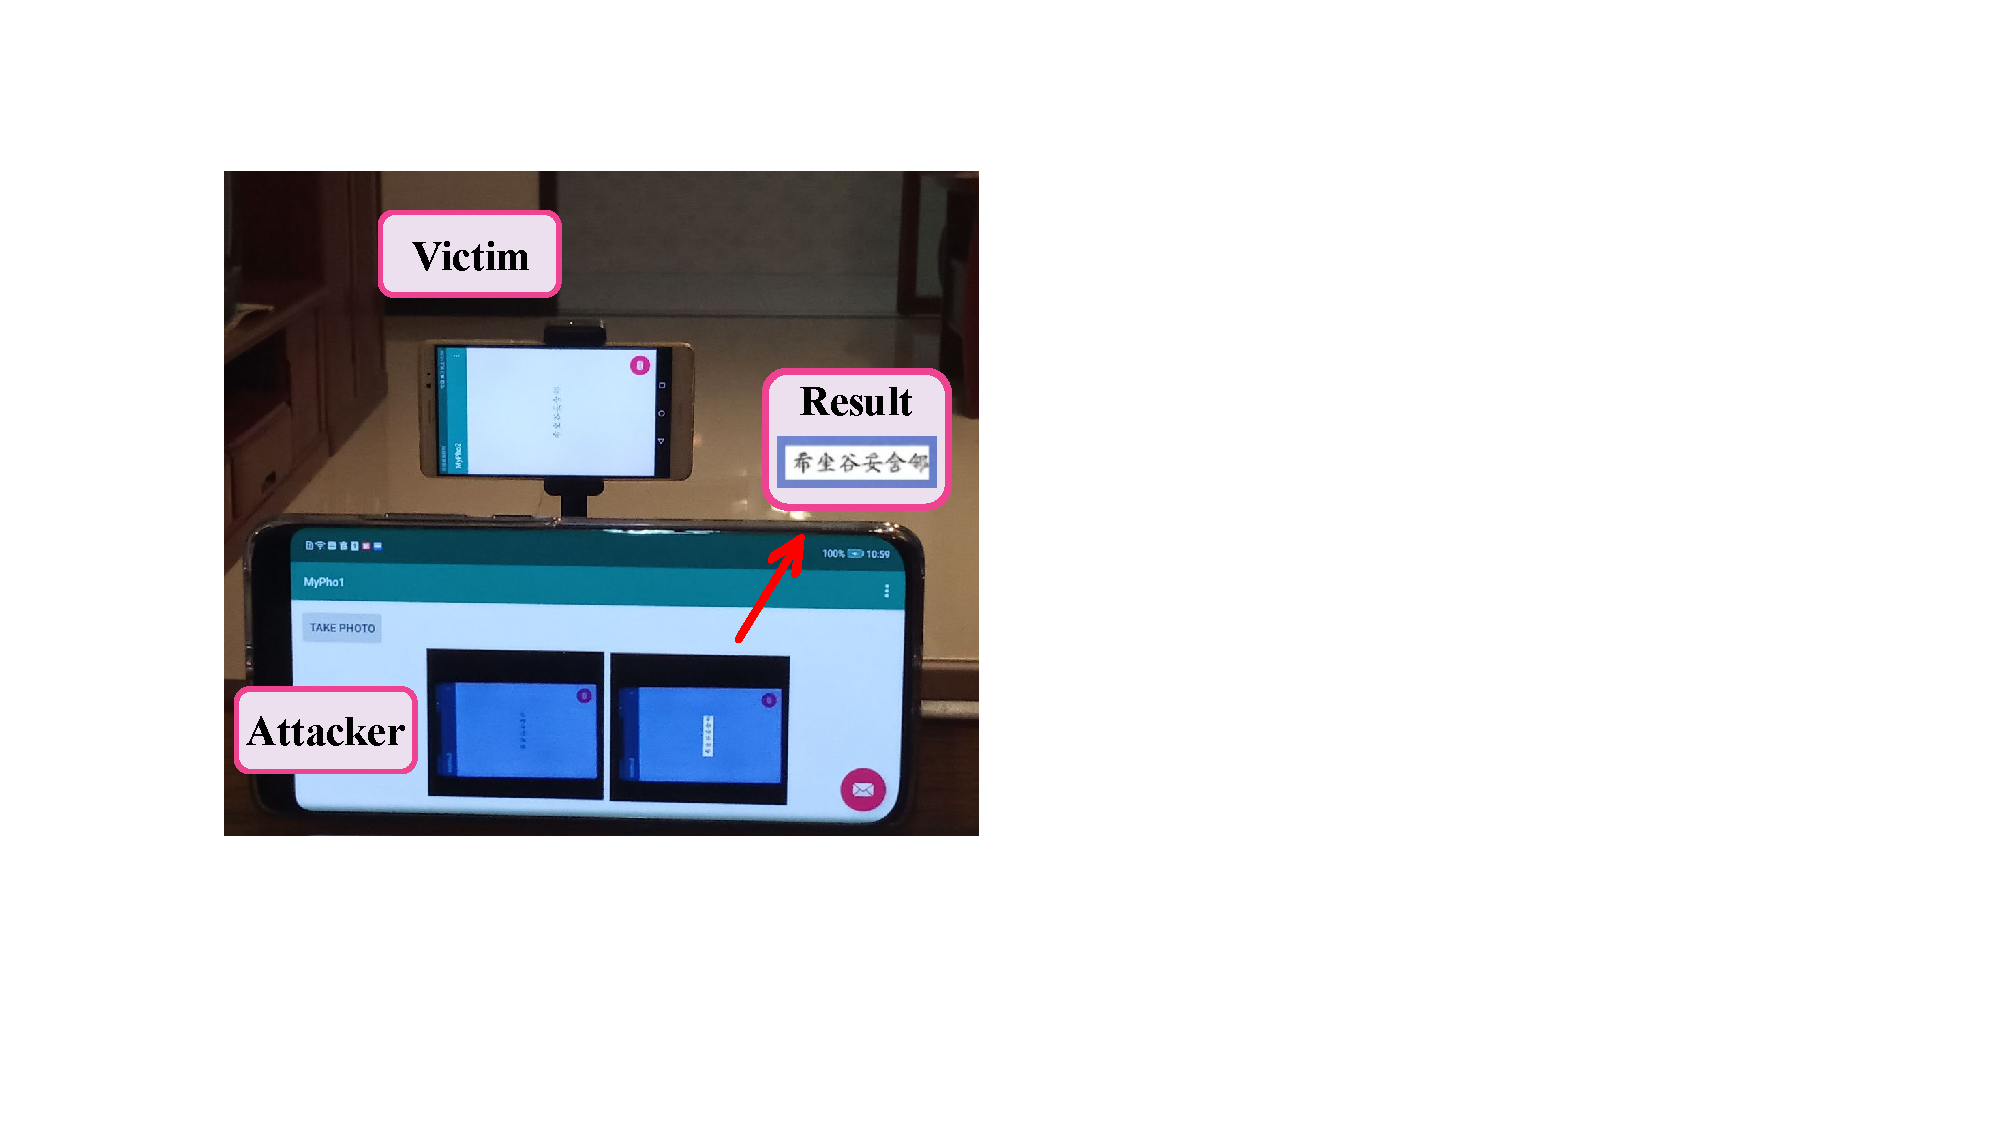
\includegraphics[width=0.46\textwidth]{pic/setup.pdf}
    \caption{Illustration of our experimental setting (Distance between phones is shortened for demonstration).}
	\label{illustration_of_system}
\end{figure}
% \begin{figure}
%   \centering
%      \centering
%      \subfigure[Experiment setting. Distance between phones are shortened for demonstration.]{
%          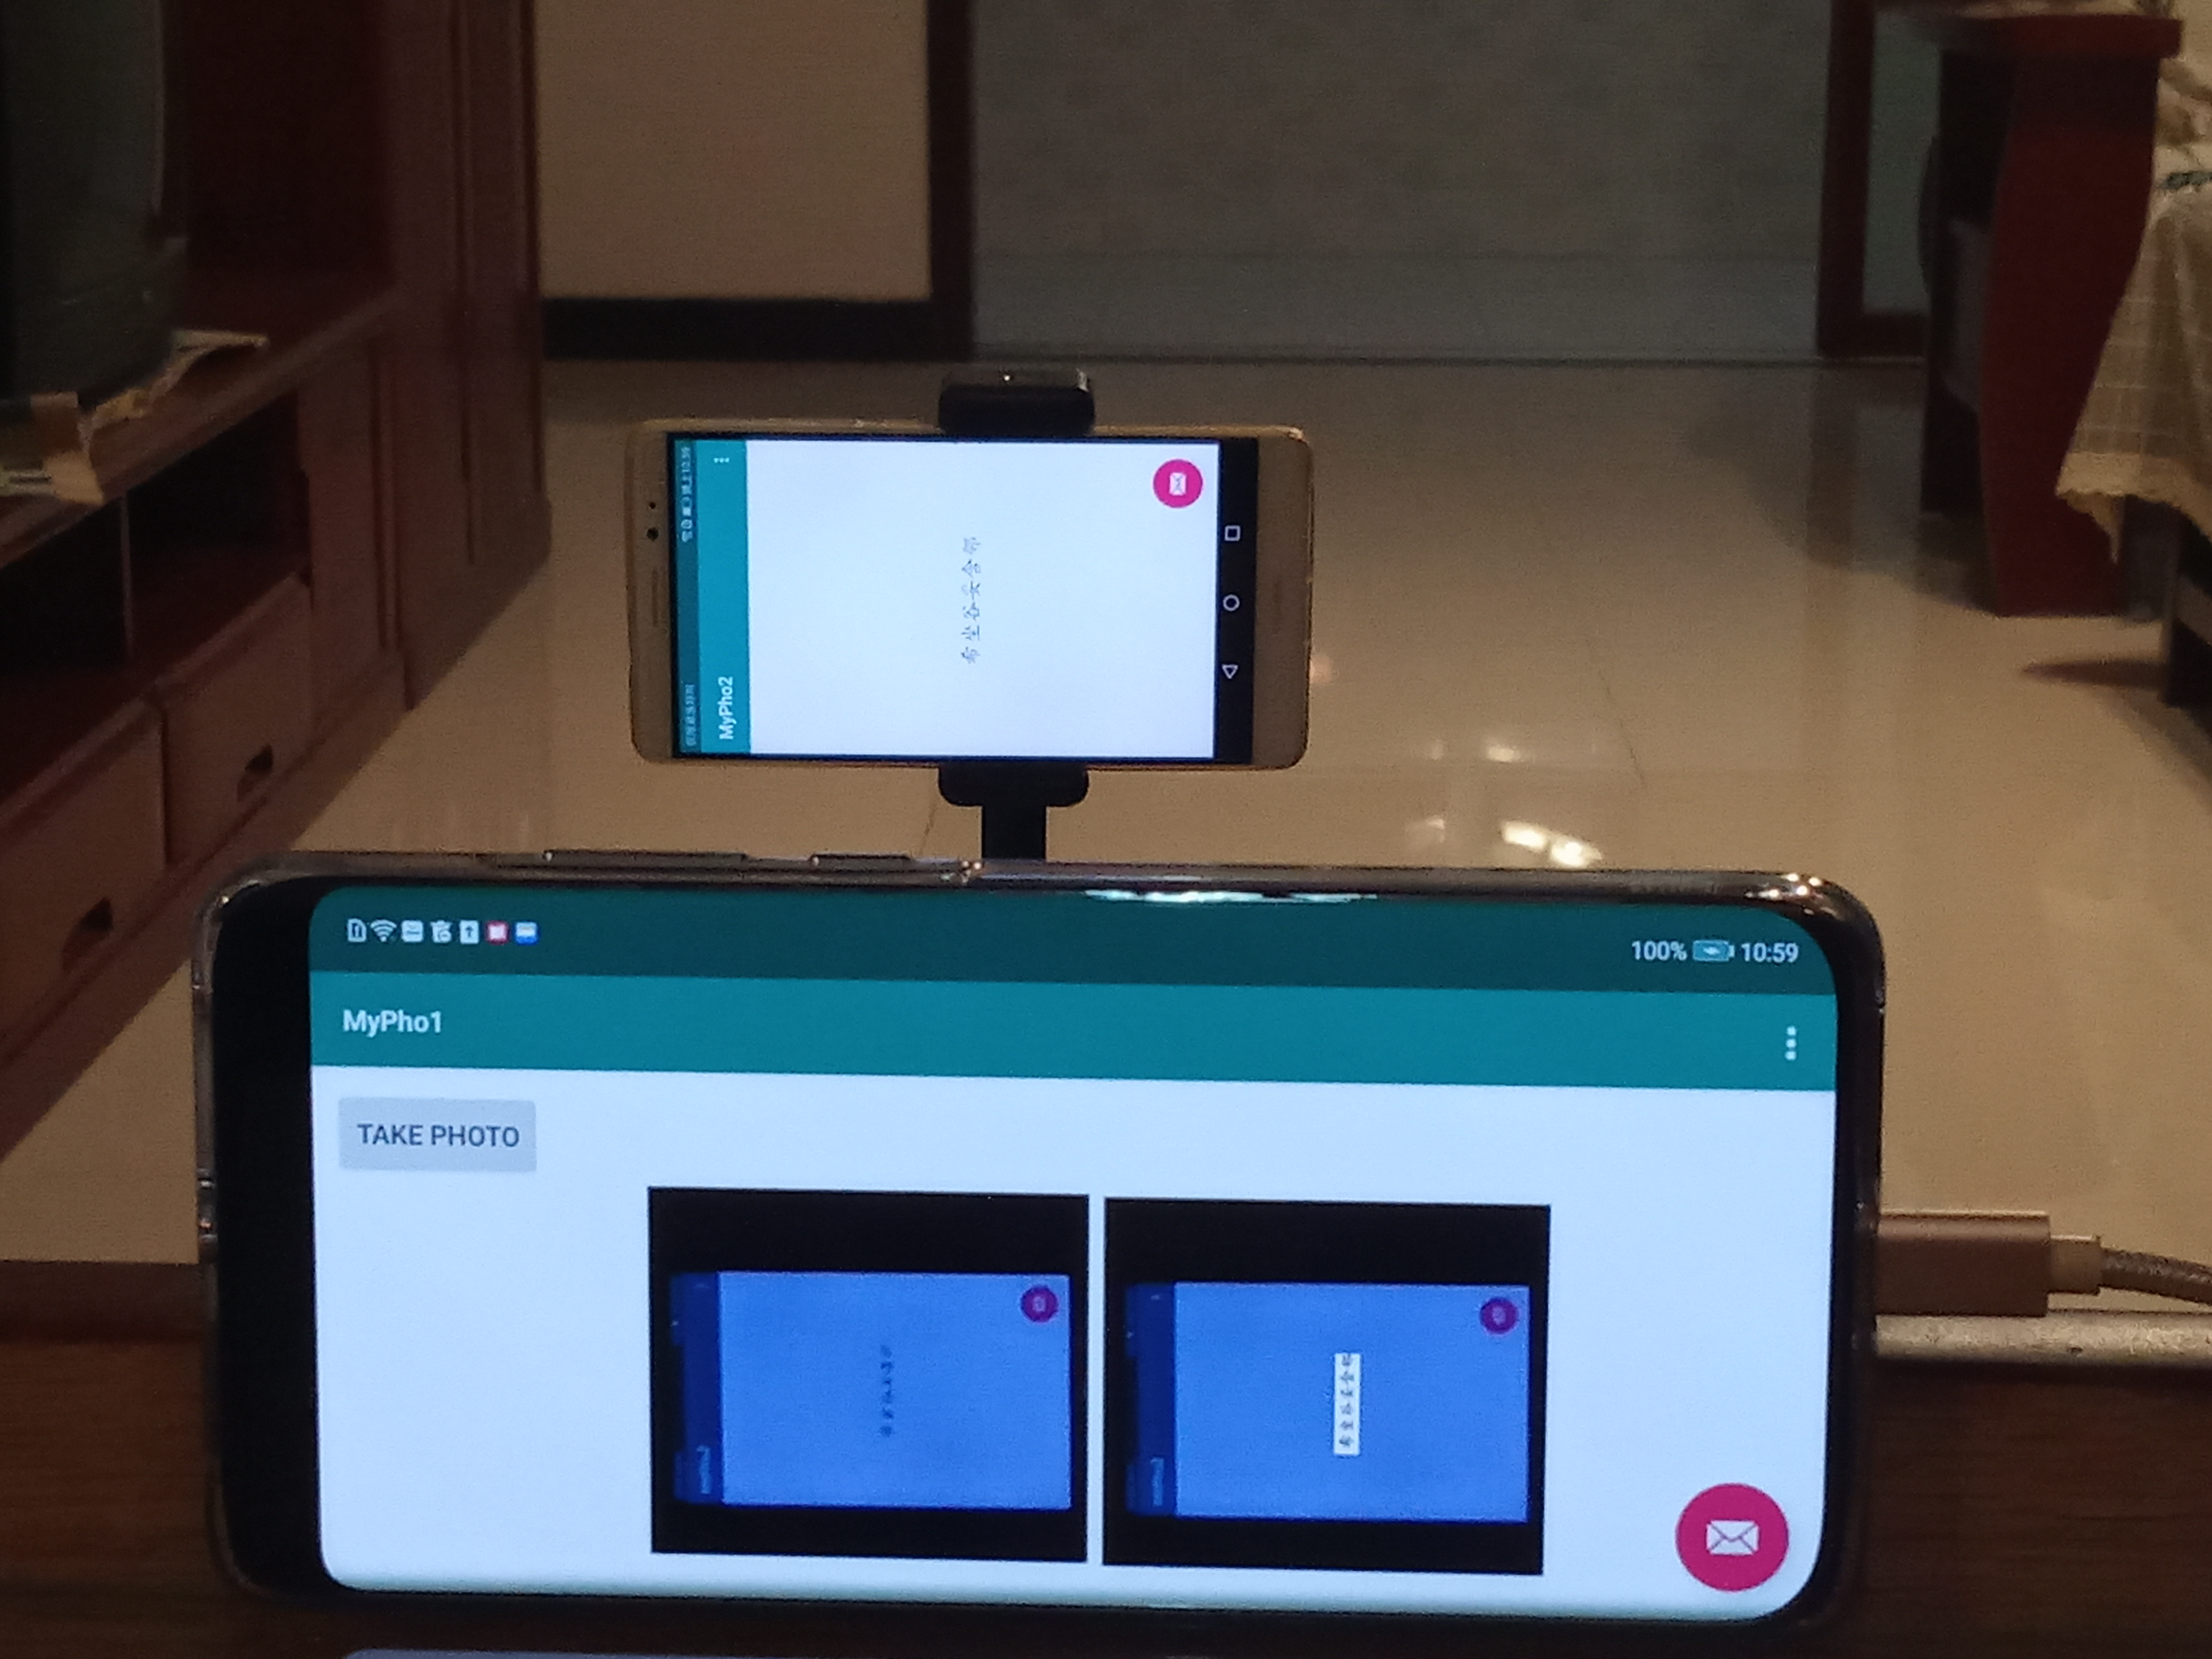
\includegraphics[width=0.5\textwidth]{pic/exp1.jpg}
%          \label{fig-exp1}
%          }
%    \subfigure[screenshot from attacker's phone(SRPeek system).]{
%          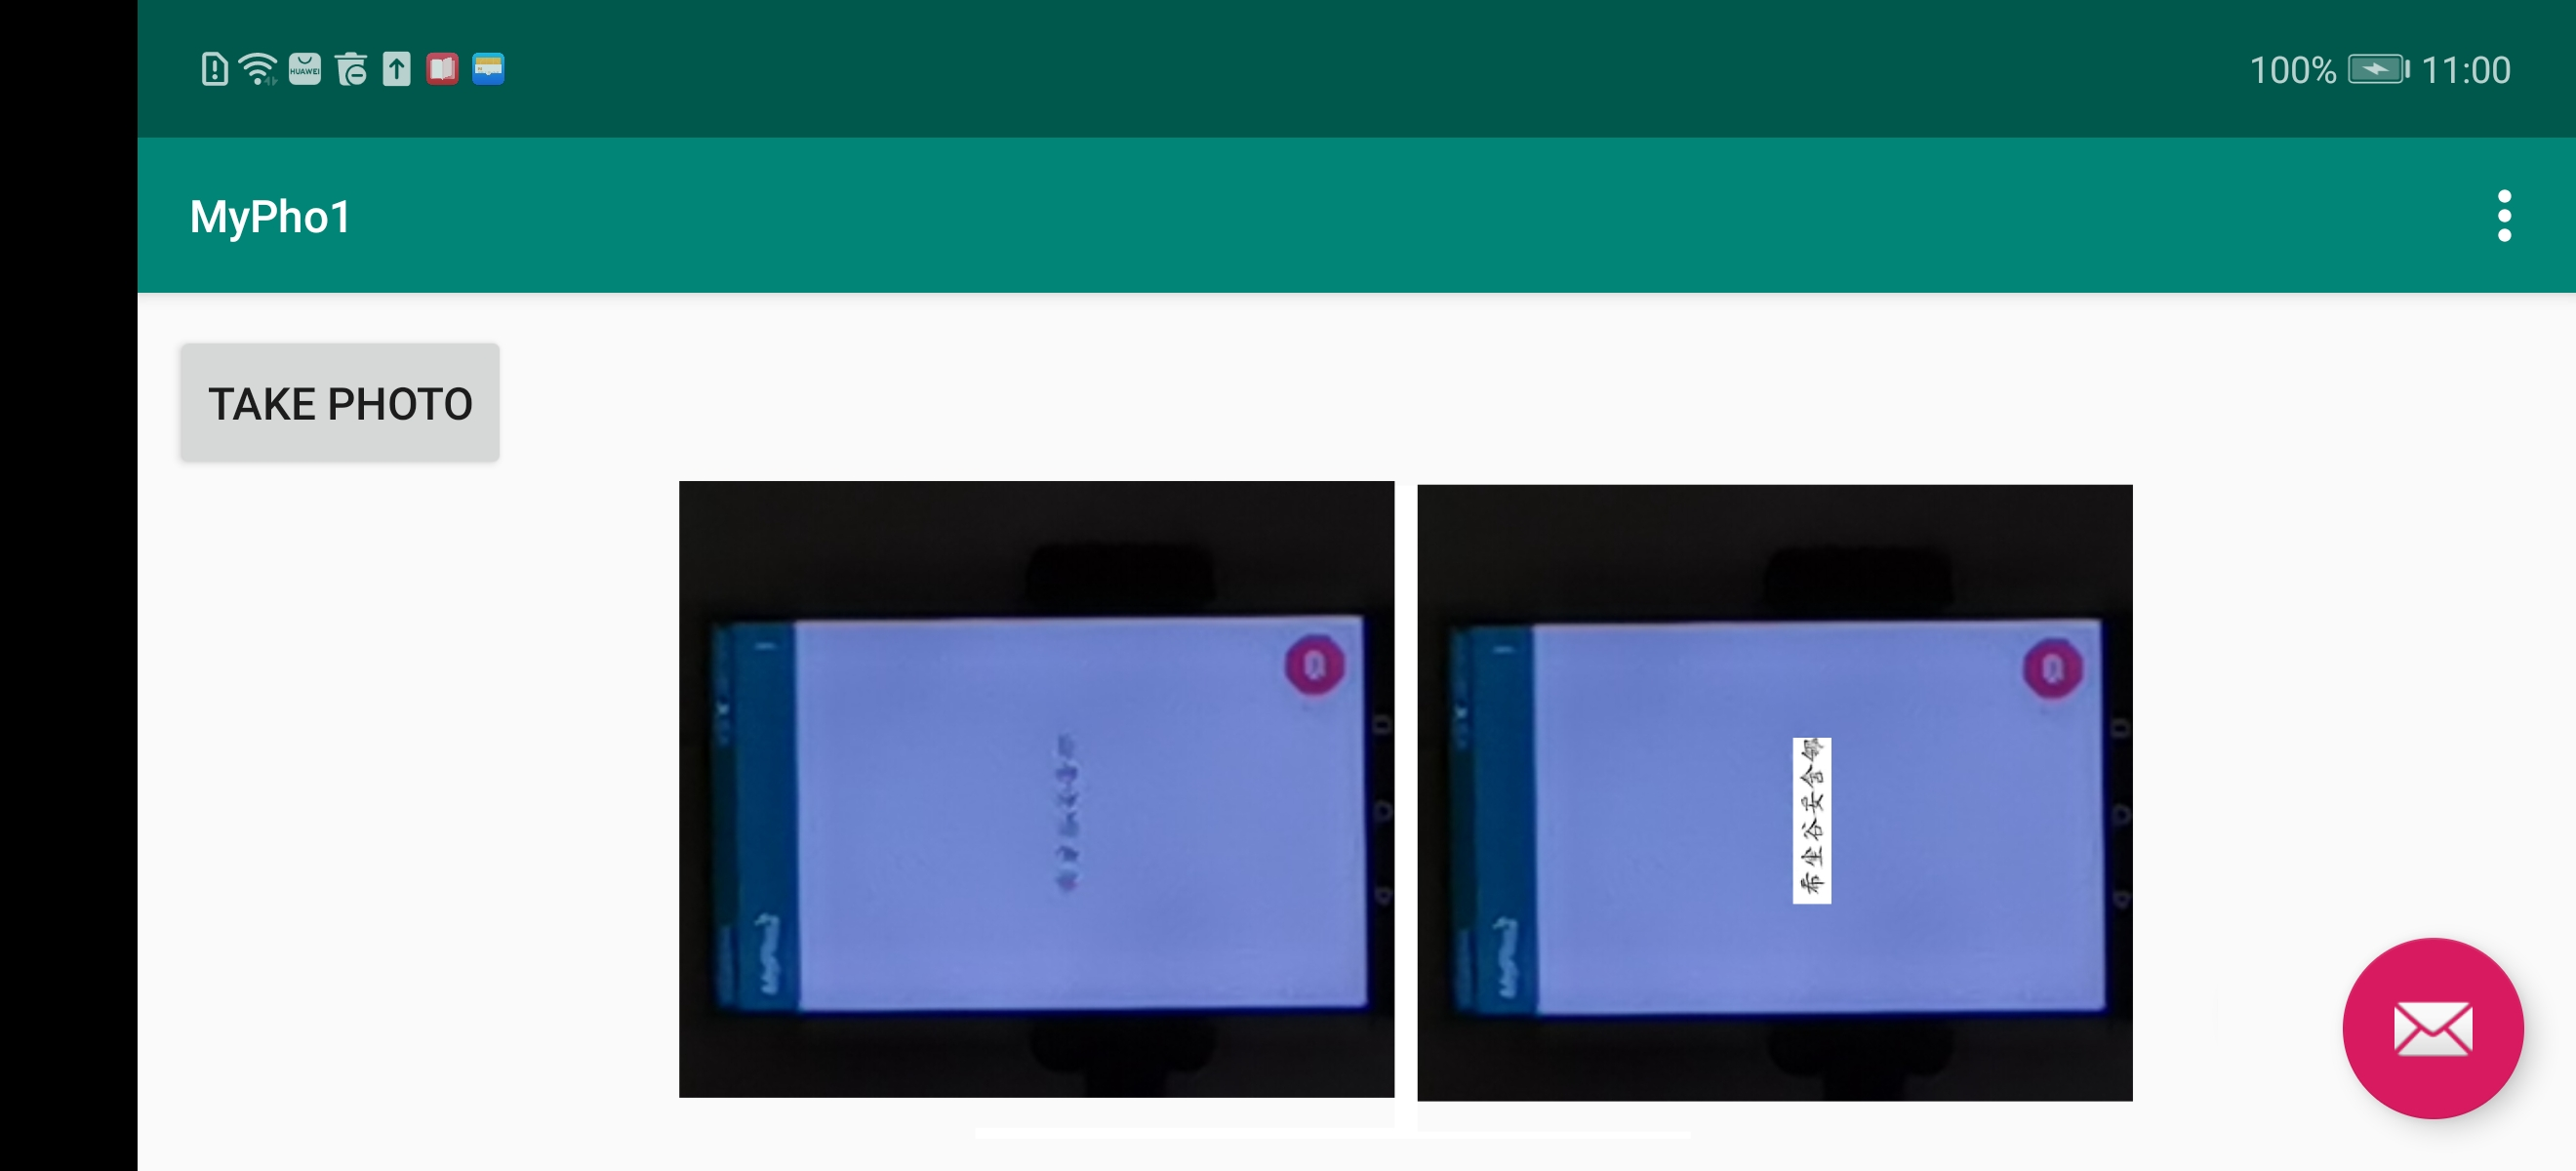
\includegraphics[width=0.5\textwidth]{pic/exp2.jpg}
%          \label{fig-exp2}
%          }
%    \subfigure[screenshot from victim's phone.]{
%          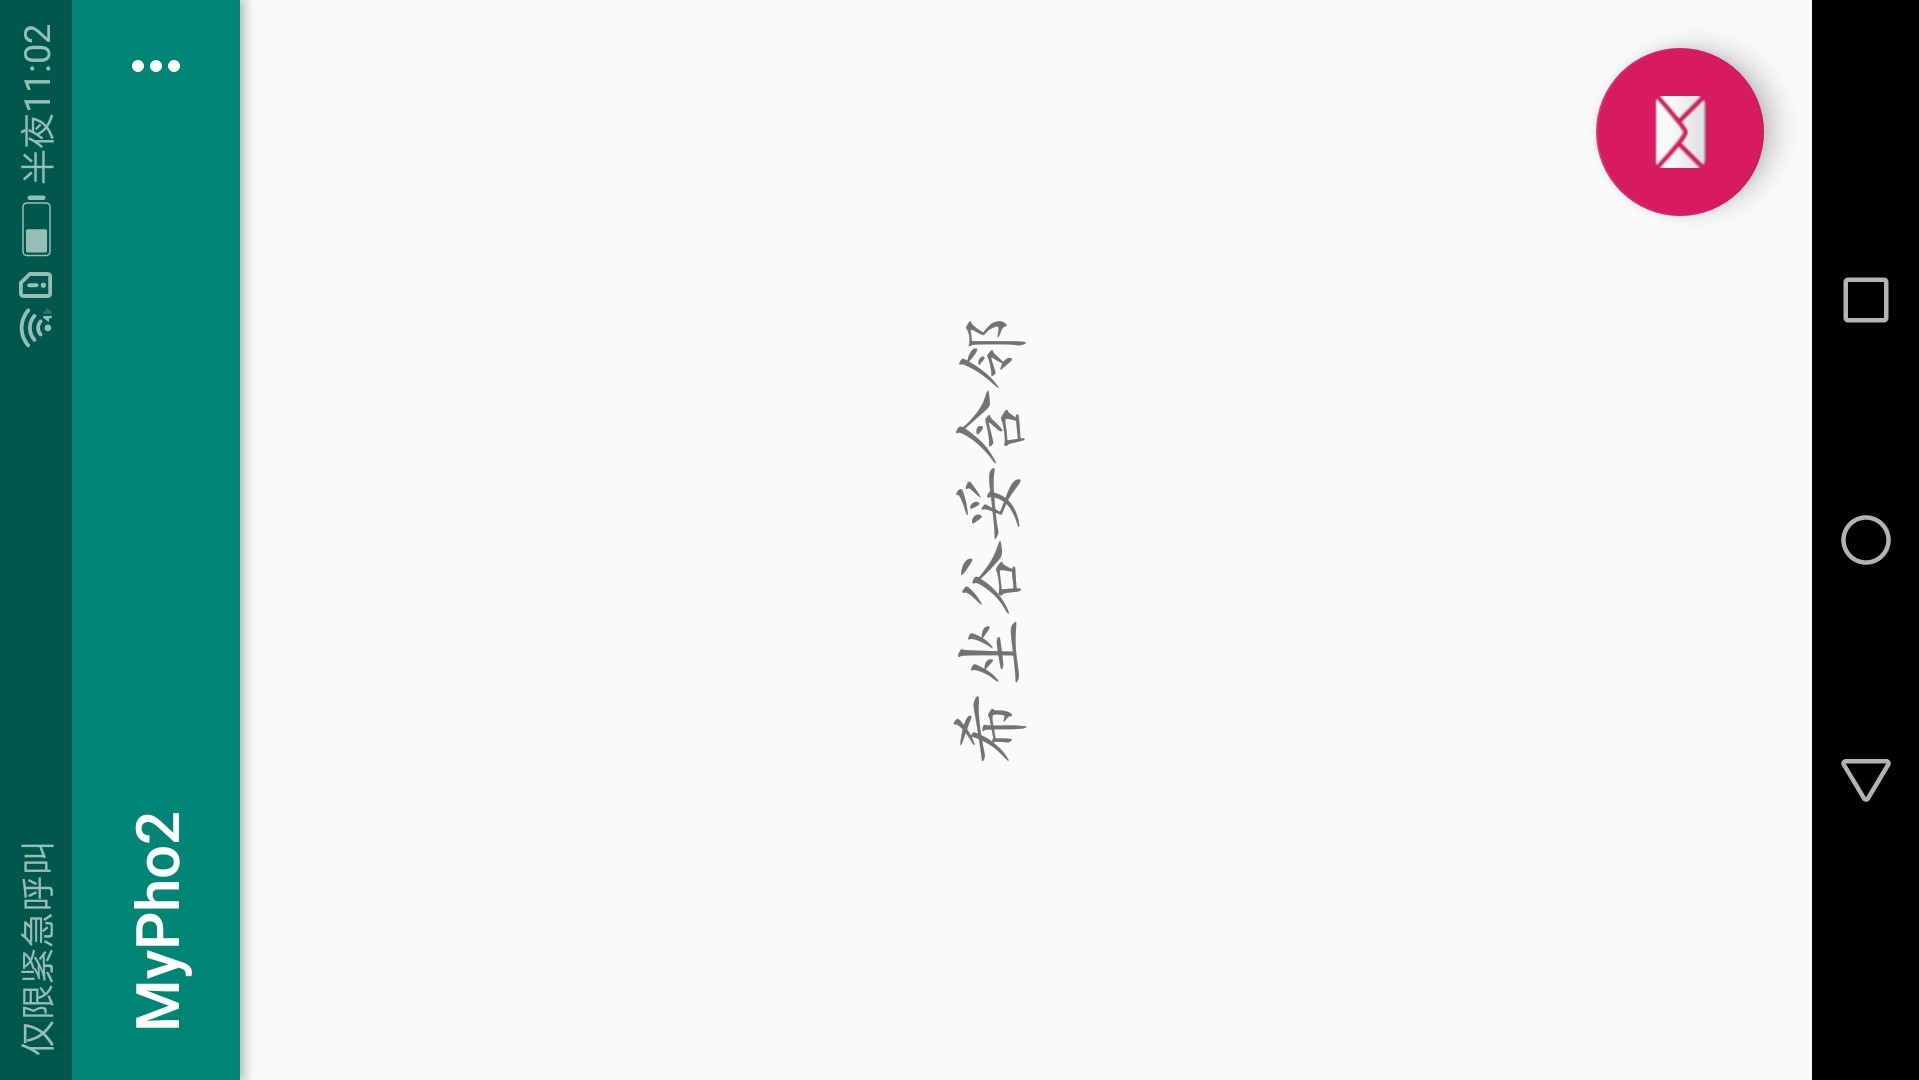
\includegraphics[width=0.5\textwidth]{pic/exp3.jpg}
%          \label{fig-exp3}
%          }
%      \caption{Illustration of our experimental setting.}
%      \label{fig-experiment}
% \end{figure}

The data was collected indoors, as is often the case of shoulder-surfing in public areas (theaters, subways, offices, etc.). We perform the experiment in a room with a window and repeat the data collection phase in different times of the day and night, with curtains drawn or open, lights turned on and off to modify the illumination parameter. The position of the phones is also a crucial factor in this parameter, and we avoid extreme settings, e.g. having the sunlight directly shining on the screen. We collected 800,000 images in this way with a Redmi6A phone (which possess a camera with 130 million pixels). This process is extremely time-consuming, but the data amount is crucial in our experiment, as slight variations of the environment will cause drastic changes in the features extracted from the characters, and only by covering the variations in each of the environmental parameters in the training data can the system successfully function in different scenarios.

\subsection{Model Specifications}
It is our observation that cameras in different phones display different patterns of distortion when performing the shoulder-surfing experiment, and apparently, images captured from a phone with weaker abilities (less pixels, less range of focus, worn lenses, etc.) will need a stronger, more complex model to extract the features. Thus, the specifications of our model are only for reference and may not work when reproduced on another phone.

Our model accepts 20 images at a time, with a size of 9x9 pixels. The model consists of 5 blocks described in the previous section. In each block, feature maps from the previous layer are passed through a single convolutional layer with 32 channels of feature maps as output. the 20x32 feature maps are then merged horizontally with the max-min-average process, and the output is 5x32 channels. Simultaneously, the original input images are processed again with a single convolutional layer with 32 channels output, and stacked with the former 5x32 channels to form a dataflow of 6x32 channels for each one of the 20 images. These channels are finally passed through a single convolutional layer, outputting 32 channels per image for the next block. The kernels in each convolutional layer is 3x3. We also insert LeakyReLU and Batch Normalization processes after each convolutional layer, and 2 upsampling layers between the 5 blocks. A single 1x1 convolutional layer is placed after the 5 blocks with a single channel as output to form the final output layer. This model consists of approximately 200,000 parameters and a complexity of about 400,000 FLOPs. As a light-weighted model, it makes a prediction within 0.1 seconds on a Tesla K80 GPU over a 9x9 patch, and when implemented on a smartphone, the human user can recognize a character within 2 seconds of processing time.

\subsection{Training Process}
Because of the difficulties in discovering the patterns among the blurry images, the training process is not so straightforward and somewhat time-consuming. Our approach is as follows: we first collect 60,000 images at a stationary experiment setting and train the model with it, as mentioned in Sec~\ref{sec-experiment-setting}, until we get satisfactory results on the test dataset. The model should be able to handle this task easily. After that, we use transfer learning methods to fine tune the model in order to fit different environmental parameters. We add a small percentage of image data from another similar experiment setting into the training data and resume training. When the model stabilizes, continue adding data from the same setting until the model can equally process data from the two image collections. Note that in this process the model will tend to extract false features, displaying wrong but clear texts as result. This phenomenon can be mitigated with dropout and normalization layers. As the model successfully fits two of the image sets, we repeat this procedure for several times until it shows signs of self-adapting, for example, when presented photos taken at 1.8m and 1.2m range in the training process, the model fits 1.5m photos easily. After that, the model can learn with the full fully-shuffled dataset with fewer difficulties.

